\chapter{Required Properties of E2E Systems\ifdraft{ (Dan) (100\%)}{}}
\label{chapter:required_properties}

In August 2010, the U.S. Election Assistance Commission issued a set
of testing requirements for UOCAVA remote electronic voting system
pilot projects~\cite{eac-uocava2010}. The general categories of
requirements specified by the EAC included functional requirements,
such as the need for the system to produce paper records of voter
choices and generate human-readable ballot images; requirements on
software development, such as allowable programming languages and
coding conventions; usability, accessibility and privacy requirements,
such as that a voter's ballot choices must remain private and that
provisions must be made to support voters with disabilities; security
requirements, including logging requirements, requirements on
communications security within the system, and requirements on
physical security and penetration resistance; quality assurance
requirements describing the testing that must be done on the systems;
and requirements about configuration management mechanisms, technical
information, and documentation to be provided by system vendors.

The EAC requirements have some serious shortcomings, one of which is
that several of the requirements seem arbitrary. For example, they
specify (in Section 2.1 of the requirements document) that the voting
system shall achieve a target error rate of no more than one in
10,000,000 ballot positions, with a maximum acceptable error rate in
the test process of one in 500,000 ballot positions, without any
justification for those numbers. They further specify (in Sections
2.1.1.1--2) that ``memory hardware, such as semiconductor devices and
magnetic storage media, shall be accurate'' and that ``the design of
equipment in all voting systems shall provide for protection against
mechanical, thermal, and electromagnetic stresses that impact voting
system accuracy'' without any guidance on how to evaluate such
accuracy or protective ability.

In addition to these shortcomings, some of the EAC requirements are
inappropriate or invalid. The most obvious example of this is the set
of requirements that mandate specific ``structured programming''
characteristics of software implementation languages (Sections 4.1 and
4.4), which seem to eliminate functional programming languages such as
Haskell and Erlang---widely used in implementing high-assurance
systems---from consideration entirely.

If these issues were addressed, the EAC requirements could serve as a
solid baseline set of requirements for remote electronic voting
systems; effectively, addressing the ``IV'' in ``E2E VIV''. However,
they are not strong enough to guarantee end-to-end verifiability,
which---as previously discussed---is essential when considering
Internet voting systems for use in real elections.  Thus, we describe
here a set of required properties for E2E VIV systems that has
significant overlap with the EAC requirements.

The set of E2E VIV requirements can be broadly divided into two
groups: \emph{technical requirements} and \emph{non-functional
  requirements}. Technical requirements are those that can be directly
addressed by the design and implementation of the system, such as
authentication requirements for voters and election
officials. Non-functional requirements are those that are imposed on
the system by external entities or where the system depends on
external behaviors outside its control, such as specific election
certification guidelines and operational procedures. Each of these
groups is itself divided into several categories, and
\autoref{fig:e2eviv_requirements_hierarchy} gives a high-level
overview of these.

\begin{figure}
\begin{center}
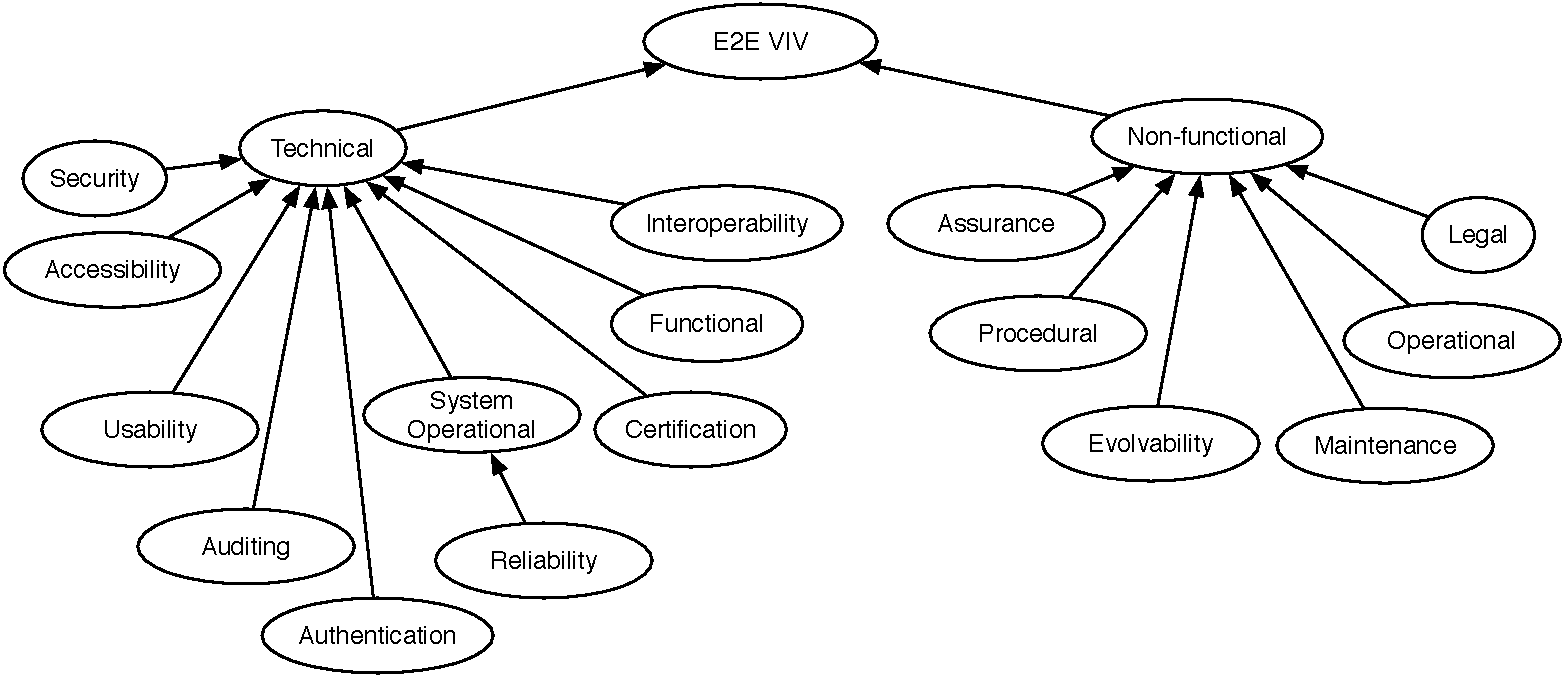
\includegraphics[width=6in]{required_properties_resources/hierarchy}
\end{center}
\caption{The hierarchy of requirements for E2E VIV systems.}
\label{fig:e2eviv_requirements_hierarchy}
\end{figure}

The following is a high-level description of the categories and many
of the requirements within each; \autoref{appendix:bon_requirements}
contains a complete listing of all E2E VIV system requirements
expressed in the Business Object Notation.

\section{Technical Requirements}
There are ten categories of technical requirements for E2E VIV
systems: functional, accessibility, usability, security,
authentication, auditing, system operational, reliability,
interoperability, and certification. 

\subsection{Functional} 
\label{sec:functional}

The functional requirements of an E2E VIV system deal primarily with
the casting and recording of ballots and associated voter records. One
important requirement is that there must be a correspondence between
the recorded ballots and the voters that are listed as having voted; a
ballot cannot be recorded without a voter casting it, and a voter
cannot be listed as having voted without casting a ballot. Similarly,
if a voter is informed by the system that her ballot has been
successfully cast, the system must correctly retain the record of her
having voted and her cast ballot information even in the event of
server failures.

Another functional requirement is the property of \emph{receipt
  freedom}: it must be impossible for a voter to prove to anybody any
information regarding how she voted her ballot, beyond what can be
mathematically deduced from the final distribution of votes. For
example, if a referendum passes with 100\% of the vote, there is no
way to hide the fact that every voter approved of the referendum;
however, if the result is mixed, it must be impossible for any
individual voter to prove how she voted.  This must be the case even
when the voter can create digital evidence of her actions by, for
example, video recording the ballot casting process or photographing a
completed ballot.

Note that there is no such E2E protocol in the literature. In order
for this requirement to be fulfilled, any protocol must allow the
voter to vote multiple times.  Yet, it must also allow it to appear
that the video-recorded vote was cast, hence its encryption must be
among those counted in a verifiable manner. Yet, this vote must not
count, and the later vote should replace it. This represents a
significant research challenge for cryptographic protocol designers.

In some elections voters are allowed to cast multiple ballots with
only the last cast ballot counting toward the final election tally,
while in others voters are prohibited from casting multiple
ballots. The system must accommodate both of these election formats,
ensuring that only the last cast ballot is counted for each voter when
multiple ballots are allowed and ensuring that each voter casts at
most one ballot otherwise.

Maintaining voter anonymity is critical, so it must be impossible
after the election to reconstruct a link between a cast ballot and any
identifying information about the voter who cast it. However, in
systems that support the casting of multiple ballots, it is important
to maintain links between voters and their ballots \emph{during} the
election to ensure that later ballots replace the correct earlier
ballots. To balance these concerns, any link between a ballot and the
voter who cast it must be irrevocably broken once it is conclusively
determined that the ballot will be counted toward the final tally.

Finally, because the voter should be able to focus on the voting
process without undue distractions or external influences, the voting
system must not display or permit the display of any advertising or
commercial logos during a voting session; the exception to this rule
is that an election jurisdiction may display its own logo to the voter
during the voting process. Along the same lines, the voting system
must not display any links to other Internet sites outside of the
voting system, except to provide help with the actual mechanics of
voting.

\subsection{Usability}

The usability of an E2E VIV system is critical to its successful
adoption and use. Since the user experience is so important, many of
the requirements of the system have some relation to usability even
though they may be categorized under other headings. There are,
however, two requirements that are exclusively related to the
usability of the system with respect to vote casting and one general
usability requirement that applies to the system as a whole.

The first vote casting requirement is that, if a voter receives a
final vote confirmation (e.g., ``Thank you for voting!'' or a similar
notice) from the system, the ballot casting process is complete and
the system has recorded the vote.  This is the usability counterpart
to the functional requirement that ballot records and voter records
must be maintained correctly even in the event of server failures.

The second vote casting requirement is that, if a voter is uncertain
whether or not her ballot was recorded (e.g., she clicked a ``submit''
button but never got a response from the system), she must be free
to attempt to vote again.

Finally, usability testing must be performed on any E2E VIV system
before it is deployed. The reports of the usability testing must be
made public, and the system must achieve satisfactory test results
before being deployed in a real election.

\subsection{Accessibility}

Accessibility---the property of being usable by and useful to voters
with disabilities---is one of the main goals of an E2E VIV system. It
is closely related to usability, but there are several requirements
associated specifically with accessibility that go beyond typical
usability requirements.

Users must be involved in the design of the system to identify
accessibility constraints at each stage of the development
process. Consideration must be given to the system's compatibility
with existing technologies designed to help individuals with
disabilities; for example, the system should be developed in a way
that allows assistive input devices such as switches, eye trackers and
screen readers to be used in addition to keyboards, mice and
touchscreens. Similarly, the system's presentation of voting options
should be optimized to voters' needs by providing alternative display
fonts, audio representations, braille representations, and other
representations as appropriate.

All possible measures must be taken to ensure that the system can be
used by all voters and, if that is not possible in all circumstances,
to provide access to alternative methods of voting for those voters
who cannot use the system.

Finally, accessibility testing must be performed in addition to the
previously-mentioned mandatory usability testing. The reports of the
accessibility testing must be made public, and the system must achieve
satisfactory test results before being deployed in a real election.

\subsection{Security and Authentication}

Security and authentication are closely related and together represent
the broadest set of technical requirements, consisting of both
requirements on the E2E VIV system itself (data storage,
communications, etc.) and requirements on the voting and counting
processes enabled by the system (voter authorization, voter privacy,
tally accuracy, etc.).

It is crucial that data integrity be ensured throughout the
system. Therefore, measures must be taken to ensure that no data can
be permanently lost in the event of a breakdown or fault affecting the
system; that the system maintains the integrity of the voters'
register, lists of candidates, ballot information, cast ballots, and
other critical information, in addition to authenticating the original
source(s) of that information and tracking provenance where
appropriate; that all data communications within the system have
associated integrity checks; that system equipment under the control
of the electoral authority is protected against influences that could
modify the election results; and that the integrity of the election
results does not depend in any way upon the security of system
equipment not under control of the electoral authority. The system
must perform regular ``health checks'' to ensure that data integrity
has been maintained, that all its components are operating in
accordance with their specifications, and that all system services are
available.

Accurate timing information is critical to security, both in terms of
providing evidence of compliance with applicable regulations and in
terms of detecting attacks on and potential breaches of the
system. The system must therefore maintain reliable synchronized time
sources, with sufficient accuracy to maintain timing data for audit
trails, election observation data, and time limits for various aspects
of the election process. It must be possible to determine, using the
timing information stored by the system, whether nominations (and, if
required, acceptance thereof by the candidate or electoral authority),
voter registration, and vote casting have occurred within the
prescribed time limits for those actions.

Authentication and authorization are also important aspects of
security. The system must ensure that each individual can be
identified uniquely, so that there is no possibility of mistaking one
individual for another. The system must also maintain the privacy of
individuals, by ensuring that all personally identifiable data is kept
confidential as far as is allowed by the legal requirements of the
electoral jurisdiction. The system must allow access to each of its
services only to authorized users; for example, only individuals who
represent the electoral authority may be allowed to load ballot
information into the system.

The authentication mechanisms used to gain access to the system must,
as far as possible, protect authentication secrets (passwords,
one-time access codes, biometrics, etc.) so that unauthorized entities
cannot acquire them. Authentication to the system may not be carried
out through third parties; that is, existing online accounts such as
those at Facebook, Google and Twitter may not be used as
authentication mechanisms. The security of the authentication
mechanism must not be affected by any potential breach of any public
or commercial database (e.g., a credit card database, the Social
Security database), and it should not be possible for an attacker to
impersonate a voter even if the entire database used for
authentication in the system is compromised. Individual authentication
secrets themselves must be changeable or revokable at any time, at the
behest of either the individual or election officials, and must be
changed for all individuals at least once in every election cycle.

With respect to the actual voting process, only eligible voters may be
allowed to cast ballots and the system must ensure that only the
appropriate number of ballots is cast by each voter. It must be
possible for a voter to verify that the system has presented her with
an authentic ballot and, in the case of remote voting, that she has a
secure connection to an official server. 

The privacy of the vote must be preserved end-to-end to the maximum
extent possible, and individual voters may not waive the privacy of
their votes. In the case of remote voting, vote privacy must be
preserved even in the presence of arbitrary malicious code on the
voter's computer (corrupted client software, key logging software or
devices, etc.). Any client software used in remote voting must not
send data to any Internet host except those associated with the E2E
VIV system or provide any information to third parties (e.g.,
Facebook, Twitter, etc.) regarding the act of voting. Any residual
information that could be used to discover a voter's choices must be
destroyed after a ballot has been cast; if a voter uses a computer
outside the control of the electoral authority to cast her vote, she
must be provided with instructions for destroying any such information
on that computer.

With respect to vote counting, the system must accurately count the
votes and the counting process must be reproducible. The system must
also maintain the availability and integrity of all information used
to generate the final tally and all information regarding the counting
process itself for as long as required. Vote tabulation must be
\emph{software independent}; it must be possible to reconstruct a
correct tally from some record even if the election system software is
compromised.

Finally, it is expected that a deployed E2E VIV system will be an
attractive target for highly-capable adversaries that wish to
influence election results or to disrupt election processes. With this
in mind, the system must be designed and tested assuming that an
adversary has a budget of US\$10 per voter per election that can be
applied toward any critical subset of votes or voters of their
choosing; thus, an E2E VIV system for use in a U.S. presidential
election would need to be designed and tested assuming that an
adversary has a budget of approximately US\$1,300,000,000.

The electoral authority shall have overall responsibility for
compliance with these security requirements, and such compliance shall
be assessed by independent bodies as appropriate.

\subsection{Auditing}

The ability to perform comprehensive audits of system activity is one
of the important distinguishing aspects of an E2E VIV system as
compared to other voting systems; as a result, there are several
system requirements related specifically to auditing, in addition to
those security requirements (such as the tracking of accurate timing
information) that touch on auditing.

First, the audit system must be designed and implemented as part of
the E2E VIV system from the beginning; it cannot be added as an
afterthought to an existing system. Audit and monitoring facilities
must be integrated into all levels of the system, from low-level
communications among individual computers to high-level interactions
with election officials. The system must keep audit logs of all
activity relevant to the conduct and outcome of the election, and
these logs must be unmodifiable once they are written and as complete
as possible without violating voter privacy.

The audit system must actively report on potential issues and threats,
rather than merely serving as a passive repository of system logs. It
must record at least the following events and actions with accurate
timing information: all voting-related information, including the
number of eligible voters and votes cast, the number of invalid votes,
count and recount results, etc.; any detected attacks on the operation
of the system or its communication infrastructure; and any system
failures, malfunctions, or other detected threats to proper system
operation. It must provide sufficient information to election
observers in real time, and after the election's conclusion, to verify
that the election is carried out in accordance with applicable
law.

The audit system must also be able to cross-check and verify the
correct operation of the voting system and the accuracy of the
election results, to detect voter fraud, and to prove that all counted
votes are legitimate and that all ballots have been counted. In
situations where the system cannot verify the legitimacy of all the
votes, it must be capable of giving an upper bound on the number of
affected ballots. If a tradeoff must be made between maintaining voter
privacy and identifying the perpetrators of fraud, the system must
resolve that tradeoff in favor of voter privacy.

In order for an E2E VIV system to be trusted, its auditability must
extend to its own source code as well as the activities it performs
during an election. Therefore, the E2E VIV system software, including
any official monitoring and auditing applications, must be published
in source form along with documentation, instructions for building and
running, and a digital signature as a proof of authenticity.

\subsection{System Operational}

System operational requirements ensure that the system is configured,
updated, and run in a transparent, accountable way that allows for the
other requirements to be fulfilled. One important such requirement is
that there must be official published manifests of the system used to
run any election, indicating details of the software and versions
used, dates of installation, and brief descriptions of their
functionality. Well-defined procedures must exist for both updating
the manifests to reflect changes to the installed software and
checking the installed software against the manifests to detect
tampering.

Before every election period, all equipment (including all software)
must be checked and approved in accordance with procedures devised by
the electoral authority. This check must include a check of the
software against the manifests, as well as any necessary tests to
establish that the system complies with its technical specification.

During an election period, key equipment must be located in a guarded,
secure area at all times. There must be a contingency plan for system
failures including provisions for backup and failover systems, which
must conform to the same standards and requirements as the systems
they replace. In addition, sufficient arrangements for data backup
must be in place, continuously monitored, and always available during
the election; election staff must be ready to intervene rapidly,
according to a procedure established by the electoral authority, in
the event of incidents during an election. Individuals responsible for
the voting equipment must follow established procedures to ensure that
the equipment and its use satisfy requirements.
 
To ensure accountability on the part of the electoral authority and
election system vendors, a report containing every software manifest
change and every violation of data security, system security, physical
security or control procedures must be prepared and made public by the
electoral authority within a reasonable amount of time after every
election.

\subsection{Reliability}

In order to be successfully used to conduct elections, an E2E VIV
system must satisfy strict reliability requirements with respect to
both its behavior under normal conditions and its behavior while under
attack.

In general, the back-end (i.e., non-voter-facing) components of the
system must have a proven mean time before failure (MTBF) of at least
one week under constant peak expected load; that is, it must have been
shown in multiple actual tests of mock elections to run continuously
for at least a week at the highest expected voter participation
rate. The one week MTBF requirement applies only during normal
operation, not while the system is under attack.

In addition to the MTBF requirement, the system must also exhibit
99.9\% uptime during the election period, and must be able to recover
from any failure other than a regional natural disaster or malicious
attack in less than 10 minutes. This must be demonstrated by inducing
failures in actual mock election situations, e.g., by unexpectedly
unplugging servers or disconnecting storage devices. Redundant
failover components must be in place for all critical components of
the system in order to ensure the 10 minute maximum recovery time.

An E2E VIV system is likely to be a tempting target for distributed
denial of service (DDoS) attacks; it must be able to continue correct
operation during a sustained DDoS attack at a specified level on any
combination of its back-end components with no more than a specified
acceptable degradation of response time to voters during the
attack. The specified attack level and acceptable degradation of
response time will vary among election types; for example, a system
running a national election must be able to resist a significantly
higher level of attack than a system running a county election. Our
initial suggestions for the thresholds for a national election are
that the system must continue operating correctly under a DDoS attack
at a level of 100 gigabits per second, with no more than a 15 second
degradation of response time.

The ability of the system to survive DDoS attacks and continue
operation while fulfilling the response time requirements must be
demonstrated in the actual network configuration to be used during the
election, and the required thresholds for these values should be
re-evaluated every election cycle to keep pace with advancement in
attack technology.

\subsection{Interoperability}

E2E VIV systems must use open, rather than proprietary, data and
communication standards for interoperability among their various
components and services. Whenever possible, the Election Markup
Language (EML) or a similar standard ratified by an international
standards body should be used for data interchange and configuration
within the system. The standards used within the system should allow
for localization of election data in situations where such
localization is required.

The log data for the system, and documentation describing its meaning
and format, must be available for public download so that anybody can
download, inspect, and publish concerns based on the system logs. 

\subsection{Certification}

In order to provide sufficient evidence for certification of an E2E
VIV system, each functional requirement must have an associated set of
automated tests that demonstrate its fulfillment. These tests must be
runnable on demand, and their results should be unambiguous and easily
understandable.

In addition, the election protocol implemented by the system
(communication, cryptographic, etc.) must have associated formal
proofs of correctness and security to the extent possible. Note that
until recent years it was rarely possible to provide proofs of
integrity properties, hence security properties that are proven
tend to be privacy properties, but this state of affairs is evolving
rapidly in the verification community.

\section{Non-functional Requirements}

There are five categories of non-functional requirements for E2E VIV
systems: operational, procedural, legal, assurance, and
maintenance/evolvability.

\subsection{Operational}
\label{req:operational}

The operational requirements on E2E VIV systems deal with several
distinct issues including election and registration timing, voter
registration, candidate nominations and lists, receipt freedom, voter
assistance, and the handling of hardware and software platform issues
and election integrity violations.

Voters must be informed, in clear and simple language, of how
electronic voting will be organized and what steps a voter will need
to take in order to participate and vote electronically. Support and
guidance with respect to voting procedures must be available to all
voters. In the case of remote voting, such support and guidance must
be available through a different, widely-available communication
channel (such as a dedicated phone number) in addition to being
available via the Internet. Voters must receive clear guidance about
exactly what client configurations (i.e., hardware platforms,
operating systems, browsers, browser plugins, other applications, and
versions thereof) are required by or supported by the E2E VIV system,
and what common components, plugins, or other software (e.g., pop-up
blockers, script blockers) may interfere with voting. In addition,
voters must receive clear guidance about configuration choices they
can make to more strongly protect their privacy; for example,
disabling cookies and browser history logging, running
privacy-protecting browser plugins, voting from temporary virtual
machines, logging out of social networks, disabling
non-election-related Internet communications, etc.

In any election carried out using an E2E VIV system, the relevant
jurisdiction's legal provisions must provide for clear timetables
concerning all stages of the election. The period during which a vote
may be cast electronically must not begin before the public is
notified of the election; in particular, with respect to jurisdictions
that allow remote electronic voting, the voting period must be defined
and made known to the public well in advance of its start. In
jurisdictions where remote voting takes place concurrently with voting
at supervised polling stations, the time periods for remote and
supervised voting need not be identical; however, remote voting should
not be allowed after the period for supervised voting has ended.

An E2E VIV system must have a publicly accessible voters' register
that is regularly updated. Each voter must be able to check, at a
minimum, that her information as recorded on the register is accurate,
and must be able to request corrections of any inaccurate
information. In jurisdictions where remote electronic voting takes
place concurrently with voting at supervised polling stations, the
system must be designed in a way such that it prevents any voter from
voting more than once.

On any electronic ballot, all voting options must be presented
equally; that is, there must be no distinguishing fonts, sizes,
styles, or other embellishments that could cause one or more of the
voting options to be perceived by a voter as ``preferred''. The ballot
must be free of any information about the voting
options---biographical information about candidates, interpretations
of and statements about ballot initiatives, etc.---other than
information strictly required for casting the vote or required by law
to be on the ballot (for example, candidate party affiliation is often
required to appear). The system must also avoid displaying any
messages that may influence voters' choices. Additional information
about voting options might be made available from an electronic voting
site as part of an E2E VIV system, separate from the actual electronic
ballot; if so, such information must be presented without bias.

E2E VIV systems are likely to be made available for testing by voters
and election officials, both before and during elections. They must
therefore indicate clearly, before the final casting of any ballot,
whether the ballot is being cast in a real election or as part of a
test. In the case of a test that occurs simultaneously with a real
election, individuals casting test ballots should subsequently be
directed to the appropriate voting channel for casting real ballots.

E2E VIV systems must exhibit receipt freedom (mentioned previously in
the technical requirements); that is, they must not enable the voter
to possess a proof of the choices they have made in a cast
vote. Receipt freedom has two different meanings, depending upon
whether or not the voting apparatus is supervised (in a polling place)
or unsupervised (as is the case in most remote voting systems).

In a supervised environment, voting information should disappear from
the display (visual, audio or tactile, depending on accessibility
requirements) used by the voter to cast the vote as soon as the vote
has been cast. When a paper proof of an electronic vote is provided to
the voter at a polling station, the voter must not be allowed to show
it to any other person or to remove it from the polling station. Note
that the only existing protocols with receipt freedom are those that
assume a private channel with the voting system and/or a trusted
voting computer. This is not necessarily a reasonable assumption in a
remote voting scenario.

In the unsupervised setting, as discussed in
\autoref\label{sec:functional} above, the situation is different,
though the underlying secure goal is the same.  Even were an
adversary/coercer were to digitally record the voting process or the
voter were to record themselves with the intention of selling their
vote, it must not be possible for the adversary to irrefutably
conclude, either during the election or after the election is
certified, that the coerced/sold vote is, in fact, as recorded.

With respect to counting the votes, an E2E VIV system must not allow
the disclosure of any vote counts until after the system has stopped
accepting electronic ballots. Tally information must not be disclosed
to the public until after the end of the voting period (including all
polling station voting). Any decoding required for the counting of the
votes shall be carried out as soon as practicable after the end of the
voting period; representatives of the electoral authority must be able
to participate in, and observers must be able to observe, the counting
process. A record of the counting process must be kept, including
timing information and identifying information for all persons
involved in the counting process. In the event of any irregularity
affecting the integrity of votes, it must be recorded that the
affected votes had their integrity violated; the effect of such
integrity violations on the election results will vary based on the
legal provisions of the involved jurisdictions.

Finally, any deployed E2E VIV system must function correctly as an
open system, where large parts (specifically, any remote client
hardware and software) are unknown, unsecured, uncertified, and
completely out of the control of election officials. The system must
be auditable to the extent possible given this requirement, and the
conclusions drawn from the audit process should be applied in future
elections.

\subsection{Procedural}

Successful deployment of E2E VIV systems requires certain procedures
to be followed with respect to their provisioning, certification,
maintenance, availability, and use. Because such systems are critical
pieces of public infrastructure, information about their functioning
must be publicly available and information about the specific
components of a system must be disclosed, at least to the relevant
electoral authority, as required for verification and certification
purposes. Before any such system is introduced, at appropriate
intervals after its introduction, and in particular when any changes
are made to the system, an independent body appointed by the electoral
authority must verify that the system is working correctly and that
all necessary security measures have been taken.

After introducing a system, the electoral authority must take steps to
ensure that voters undesrtand its use and have confidence in the
system; these may include outreach, practice elections, and any other
measures the electoral authority sees fit. In particular, voters must
be given an opportunity to practice any new electronic ballot casting
method before, and separately from, the casting of an electronic
ballot during a real election.

The electoral authority must take steps to ensure the reliability and
security of the E2E VIV system; for example, guarding equipment,
providing suitable reliable power supplies, etc. All possible steps
should be taken to avoid the possibility of fraud or unauthorized
intervention during the voting process, and the electoral authority
must satisfy itself that the E2E VIV system is genuine and operates
correctly before using it to conduct a real election. 

Only individuals appointed by the electoral authority should have
access to the central infrastructure, the servers, and the election
data, and clear rules should be established for such
appointments. Critical technical activities must be carried out by
teams of at least two people, and the composition of such teams must
be regularly changed. As far as possible, critical technical
activities should take place outside of election periods. 

Observers must be allowed to be present, to the extent permitted by
law, to observe and comment on the conduct and establishment of the
results of any election conducted using an E2E VIV system. During an
election period, any authorized intervention affecting the system must
be carried out by a team of at least two people, be the subject of a
written report, and be monitored by representatives of the election
authority and election observers.

The system must maintain the availability, integrity, and
confidentiality of the votes. It must also keep the votes sealed until
the counting process begins. Any votes stored or communicated outside
controlled environments must be encrypted. Recounts must be possible,
and any features of the system that may influence the correctness of
the result must be verifiable. The system must also support partial or
complete re-runs of elections. 

Finally, there must be clear technical and legal procedures to be
followed in the event that voters can prove that their votes were not
received accurately or counted, or in the event that the official
election verification application does not verify that the results of
the Internet portion of the election are correct.

\subsection{Legal}

Legal requirements arise primarily from the application of existing
law to E2E VIV systems. These include requirements on accessibility
and availability; on the counting of votes, number of votes per voter,
and anonymity of votes; and on restrictions with respect to reverse
engineering or testing of E2E VIV systems.

To comply with accessibility and availability requirements, the voting
interface of an E2E VIV system must be understandable and easily
usable, and registration requirements for electronic voting must not
pose an impediment to voter participation. E2E VIV systems should be
designed, as far as is practicable, to maximize the opportunities they
provide for voters with disabilities. Unless remote electronic voting
channels are universally accessible, they must be used only as an
additional and optional means of voting beyond polling places or more
traditional remote voting methods.

The E2E VIV system must insure that at most one electronic vote from
each voter is included in the final tally, that every vote cast
electronically is counted, and that each vote cast electronically is
counted only once. In jurisdictions where electronic and traditional
voting channels are used in the same election, there must be a secure
and reliable method to aggregate all votes, prevent multiple votes by
the same voter from being counted, and calculate correct results.

The way in which voters are guided through the process of electronic
voting should be designed to prevent their voting precipitately or
without reflection. Voters must be able to alter their choices at any
point during an electronic voting process before casting their vote,
or to stop the voting process, without their previous choices being
recorded or made available to any other person under any
circumstances. The electronic voting system must not permit any
manipulative influence to be exercised over the voter during the
voting process, must provide the voter with a means of participating
in the election without exercising a preference (e.g., by casting a
blank ballot), must indicate clearly to the voter when the voting
procedure has been completed, and must preserve voter anonymity.

There must be no legal impediments to interested parties who want to
study the E2E VIV system. In particular, no nondisclosure agreement or
contract of any kind may be required for such download and study, or
for building, testing and publishing test results for the E2E VIV
system.

\subsection{Assurance}

There are several assurance requirements with respect to the
implementation, documentation, and licensing of E2E VIV
systems. First, client side software---that is, any software that is
expected to be used on a system serving as a voting terminal, whether
a supervised machine at a polling place or an unsupervised machine
belonging to a voter---must be free of known bugs on a wide range of
platform and software stack combinations. As previously discussed in
\autoref{req:operational}, the specific supported platform and
software stack combinations for the software must be clearly conveyed
to voters. The system must exhibit strong security with respect to
voter authentication, such that there is no way to automate forging or
invalidation of voter authentication credentials without compromising
the cryptographic protocols or secrets used in the system.

All aspects of the design, architecture, algorithms and documentation
for the entire Internet voting system (not just the E2EV core) should
be published and available for free download by anyone. As the system
changes, all associated documentation must be kept up to date, and no
new version of an E2E VIV system should be certified until it has
up-to-date documentation. 

The source code, build scripts, issue tracking system, security
features, and related development information for the entire Internet
voting system---all versions, for all supported platforms---should be
made publicly available for free download and inspection, under a
license that permits anyone to download, build, instrument, and test
the system.

\subsection{Maintenance and Evolvability}

Maintenance and evolvability requirements are closely related, and
essentially stipulate that an electoral authority, or any entity
engaged by an electoral authority, must be able to change an E2E VIV
system in response to changes in the legal or technical environment in
which it operates. 

The electoral authority must have the right and the ability to update
the election system to conform to changes in applicable law, available
technology, or threats to system integrity independent of the original
vendors of the system. The electoral authority must also have the
right and ability to patch election systems to correct flaws
discovered in the algorithms, implementation, or deployment, subject
to the documentation update requirement described above and the
procedural requirement that the system must be re-verified for correct
operation before being used to conduct a real election.
